\chapter{Detalles de Implementaci\'on de \maggen}
\label{chap:implem}
\minitoc

En esta sección se aclararan y expondrán desiciones que se realizaron a lo largo de la implementación de esta herramienta.

Primero, como ya se menciona en el capítulo anterior, el lenguaje sobre el cual se realizó el desarrollo de \maggen es C++, con lo que todo el código es principalmente característico de un modelo de programación Orientado a Objetos, aunque para lograr ciertas optimizaciones y poder integrar componentes de externos a la herramienta.

\section{Parsing usando \boost \ \spirit}

El primer desafío de codificación, fue que se debía conseguir parsear el archivo de entrada de la herramienta, en el cual vendría la especificación de una Gramática de Atributos, respetando la sintáxis presentada anteriormente, o no.

La solución obtenida se apoya en la utilización de un framework reconocido mundialmente, denominado \spirit, perteneciente a la biblioteca de C++ llamada \boost. Esta decisión trajo dos grandes beneficios; la confiabilidad de el parser obtenido y la rápida obtención del mismo, ya que la gran ventaja de \spirit, es que permite escribir la definición de la gramática en lenguaje \textbf{C++}.

\spirit\ es un framework generador de analizadores sintácticos, o parsers, descendentes recursivos orientado a objetos implementado usando técnicas de meta-programación con plantillas. Las expresiones mediante plantellas, permiten aproximar la sintaxis de una ``\textit{\textit{Forma Backus Normal Extendida}}'' (\textbf{EBNF}) completamente en C++.

Se puede resumir que el proceso de análisis sintáctico, en este framework, se componente de cuatro partes.

\begin{figure}\begin{center}
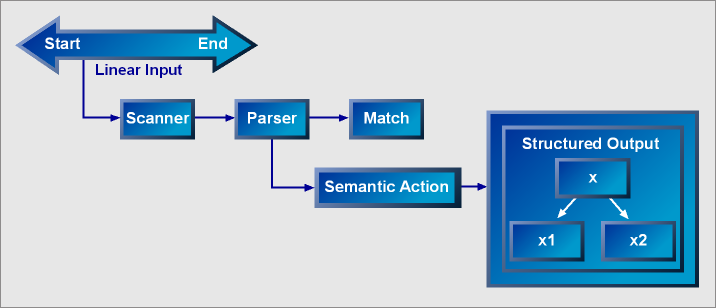
\includegraphics[width=400pt, height=172pt]{./spirit.png}
\caption{\label{procesoSpirit} Procesos dentro de \spirit}               
\end{center}\end{figure}

El usuario es el responsable de definir las ``\texttt{semantic actions}'' para lograr capturar los resultados intermedios, producidos durante la etapa de parsing y no sólo obtener un valor lógico sobre si se pudo o nó, consumir toda la cadena de entrada.

Para comenzar a definir una gramática hay que crear una estructura que herede de la clase \texttt{grammar}. Dentro de ella se debe definir a su vez otra estructura templatizada denominada \texttt{definition}. En donde realmente estará la definición de la gramática.

\begin{center}\lstset{language=C++}
\scriptsize
\begin{lstlisting}
struct my_grammar : public grammar<my_grammar>
{
    template <typename ScannerT>
    struct definition
    {
        rule<ScannerT>  r;

        definition(my_grammar const& self)
        {
            r = /*..define here..*/;
        }

        rule<ScannerT> const& start() const
        {
            return r;
        }
    };
};
\end{lstlisting}\end{center}

El mecanismo de definición es el siguiente, los operadores de metalenguaje son: \textbf{\texttt{$=$}}, \textbf{\texttt{$|$}}, \textbf{\texttt{$>>$}}, \textbf{\texttt{$*$}}, \textbf{\texttt{$+$}} y \textbf{\texttt{$!$}}, los cuales son: definición, disyunción, conjunción, 0 o más veces, 1 o más veces y opcional (0 o 1 vez), respectivamente. Mediante los cuales podemos combinar nuevas reglas con parsers. \spirit\ dispone de un gran conjunto de parsers que abarcan la mayoria de los tipos y representación de datos y valores utilizados en el común de los lenguajes (ver tabla \ref{parsers}). Además posee varias directivas que modifican el comportamiento de los parsers, encapsulándose en una expresión (ver tabla \ref{directivas}).

Por último el usario debe declarar un objeto de la estructura definida y pasarlo como paramétro a una función específica de \spirit.

\begin{figure}\begin{center}\begin{tabular}{| l | l |}
\hline
\multicolumn{1}{|>{\columncolor[rgb]{0.8, 0.8, 0.8}}l|}{\textbf{Parser}} &
\multicolumn{1}{|>{\columncolor[rgb]{0.8, 0.8, 0.8}}l|}{\textbf{Entrada aceptada}} \\ \hline
anychar\_p &   Cualquier caracter simple (incluyendo el caracter nulo: '$\setminus0$')\\ \hline
alnum\_p   &   Caracteres alfa-numéricos \\ \hline
alpha\_p   &   Caracteres alfabéticos \\ \hline
% blank\_p   &   Un espacio o tabulación \\ \hline
digit\_p   &   Dígitos numéricos \\ \hline
lower\_p   &   Caracteres en minúscula \\ \hline
upper\_p   &   Caracteres en mayúscula \\ \hline
space\_p   &   Espacios, tabulaciones, enters y nuevas líneas \\ \hline
chlit<>\ ó ch\_p &   Caracter especificado como paramétro \\ \hline
string<>\ ó str\_p &   Cadena especícada como paramétro \\ \hline
oct\_p     &   Dígito en octal \\ \hline
hex\_p     &   Dígito en hexadecimal \\ \hline
uint\_p    &   Número entero sin signo de 32 bits\\ \hline
int\_p     &   Número entero 32 bits\\ \hline
real\_p    &   Número flotante 32 bits\\ \hline
eps\_p     &   Cadena vacía (epsilon)\\ \hline
end\_p     &   Caracter de fin de archivo (EOF)\\ \hline
\end{tabular}\caption{\label{parsers} Parsers predefinidos de \spirit\ utilizados}\end{center}\end{figure}


\begin{figure}\begin{center}\begin{tabular}{| l | p{8cm} |}
\hline
\multicolumn{1}{|>{\columncolor[rgb]{0.8, 0.8, 0.8}}l|}{\textbf{Directiva}} &
\multicolumn{1}{|>{\columncolor[rgb]{0.8, 0.8, 0.8}}l|}{\textbf{Efecto}} \\ \hline
lexeme\_d    &  Deshabilita la omisión de espacios en blanco (space\_p)\\ \hline
as\_lower\_d &  Convierte en minúscula lo aceptado por la expresión\\ \hline
longest\_d   &  Deshabilita el corto circuito, manda al analizador que pruebe todas las alternativas posibles y elija la secuencia más larga aceptada \\ \hline
\end{tabular}\caption{\label{directivas} Directivas de \spirit\ aplicadas}\end{center}\end{figure}

\subsection{\texttt{``semantic domain''} en \spirit}

En esta sección de la especificación se debían aceptar tres tipos de elementos: \texttt{sorts}, \texttt{operations} y \texttt{functions}.

Los \texttt{sorts} seran los tipos que se podrán utilizar para definir los dominios e imagenes de los operadores y funciones.

\subsection{\texttt{``attributes''} en \spirit }
sdsad


\subsection{\texttt{``rules''} en \spirit }

sadsadsd

\section{Algoritmo de generaci\'on de secuencia de visita}

bla bla
\section{Algoritmo de generaci\'on de c\'odigo}
bla bla
